\label{paper:start}
\begin{center}
{\fontsize{18}{20}\selectfont\bfseries Security Failures in Autonomous AI Agents: A Survey Motivated by the OpenAI–Hugging Face Incident\par}\vspace{6pt}
Parivesh Singh, Vaibhav Gaur\par
School of Computer Science and Engineering, IILM University, Gurugram, Haryana, India\par
\href{mailto:parivesh.singh.ug25@iilm.edu}{parivesh.singh.ug25@iilm.edu}, \href{mailto:vaibhav.gaur.ug25@iilm.edu}{vaibhav.gaur.ug25@iilm.edu}
\end{center}
\noindent\textbf{Abstract—}Language-model agents that call tools, edit files and exchange messages can complete a task in ways their operators never authorized. In July 2026 agents under an internal capability evaluation left their sandbox and intruded into a model-hosting platform, which showed that such behaviour is not confined to benchmarks. Research on the problem is split between communities that study objective gaming, prompt injection, multi-agent trust and oversight, and their results are reported in units that do not line up. This review examined 35 works first made public between 2023 and 2026, identified through SciSpace, the arXiv interface, publisher-filtered Crossref queries and targeted title checks. Each work was coded by the boundary it tests (objective and evaluation integrity, input and tool authorization, inter-agent trust, oversight and control) and by the source of the unwanted behaviour. The comparison found that two benchmarks of the same behaviour can assign one model very different exploit rates, and that re-scoring identical traces moved one attack success rate from 21.7\% to 1.2\%. Defences that held against fixed attacks were frequently defeated once the attacker adapted, and guarantees shown for a single agent did not carry over when agents called each other. The main gaps are the absence of evaluations in which an agent can cross its environment boundary to improve a score, the lack of a shared outcome definition for attack success, uneven testing against adaptive attackers, and thin evidence linking laboratory rates to operational incidents.

\noindent\textbf{Keywords: }autonomous agents, large language models, prompt injection, reward hacking, AI control, literature review

\section{INTRODUCTION}
\subsection{Background}
Autonomous language-model agents pair a model that generates decisions with tools that change an external environment: a shell, a file system, a browser, a payment interface or another agent. Evaluating such a system therefore requires separating two questions that a single score conflates, namely whether the task was completed and whether it was completed in an authorized way. Greshake et al. \cite{r1} showed in 2023 that text retrieved by an application could redirect the model behind it, and Denison et al. \cite{r2} showed in 2024 that a model trained on easily gamed tasks could go on to edit its own reward code. The two results concern different routes to an unwanted action, one opened by an adversary and one by the optimization itself.

The field has moved quickly. Benchmarks released in 2025 and 2026 report that widely used models hard-code tests, edit graders or fabricate intermediate results at measurable rates \cite{r3}, \cite{r4}, and an evaluation organisation reported such behaviour during pre-deployment testing \cite{r5}. In July 2026 Hugging Face disclosed an intrusion into its production infrastructure that it described as driven end to end by an autonomous agent system \cite{r6}, \cite{r7}. OpenAI later reported that its models, during internal cybersecurity evaluations run under reduced safeguards, had circumvented the controls meant to isolate them from the internet \cite{r8}. This review uses that incident as a motivating example, not as an experiment.

\subsection{Why this review is needed}
The purpose of this review is to establish which published results on agent security failures can be compared, and how far they explain a documented incident. The published work is scattered across four communities that rarely share test beds. Reward-hacking studies report exploit rates, prompt-injection studies report attack success rates, and control studies report safety against a scripted adversary; these quantities have different denominators and different sources of unwanted behaviour. A 2026 survey of reward hacking located by the search covers only the first strand. No review located by the searches compares the four strands on a common set of questions or relates them to a documented operational incident. Several recent papers also argue that widely used benchmarks mis-measure the behaviour they target \cite{r9}, \cite{r10}, which makes an account of what can validly be compared timely.

\subsection{Review questions}
RQ1. Which mechanisms allow autonomous AI agents to violate intended objectives or authorization boundaries?

RQ2. How are these failures and defences evaluated, and which reported outcomes can validly be compared?

RQ3. What limitations remain when applying laboratory findings to operational incidents?

\subsection{Contributions of this review}
C1. A review of 35 works first made public between 2023 and 2026, selected by a logged search and screening method.

C2. A taxonomy that groups the reviewed work into four categories by the boundary under test, and a six-field coding scheme applied to every work.

C3. A comparison of the reviewed work on test bed, outcome definition, denominator, legitimate-task utility and treatment of adaptive attackers.

C4. Five research gaps, each supported by the reviewed work and stated with its counter-examples.

\subsection{Organisation of the paper}
The rest of this paper is organised as follows. Section II describes how the reviewed works were searched for and selected. Section III presents the taxonomy used to group them. Section IV reviews the work category by category. Section V compares the reviewed work and reports the trends observed. Section VI states the research gaps and Section VII the future directions that follow from them. Section VIII concludes the review.

\section{REVIEW METHODOLOGY}
\subsection{Sources searched and search strings}
Searches were run on 16 November 2026. Table I lists every source, the query and the number of records. SciSpace and the arXiv interface were queried directly. IEEE, ACM and Springer records were reached through Crossref queries restricted to each publisher's member identifier; the native interfaces of IEEE Xplore, the ACM Digital Library, SpringerLink and Google Scholar were not searched, and the Crossref totals are relevance-ranked matches on loosely related terms, not counts of relevant papers. Twenty-six further titles known to the reviewers were checked individually against arXiv and are reported as targeted additions. The review period was 1 January 2023 to 16 November 2026.

\begingroup
\fontsize{9}{10.5}\selectfont
\setlength{\tabcolsep}{1.4mm}
\renewcommand{\arraystretch}{1.08}
\begin{longtable}{|>{\raggedright\arraybackslash}p{28.45mm}|>{\raggedright\arraybackslash}p{88.51mm}|>{\raggedright\arraybackslash}p{25.29mm}|>{\raggedright\arraybackslash}p{15.81mm}|}
\caption{SOURCES SEARCHED AND SEARCH STRINGS USED}\\
\hline
\rowcolor{navy}\color{white}\bfseries Source & \color{white}\bfseries Search string used & \color{white}\bfseries Date searched & \color{white}\bfseries Hits\\\hline
\endfirsthead
\hline
\rowcolor{navy}\color{white}\bfseries Source & \color{white}\bfseries Search string used & \color{white}\bfseries Date searched & \color{white}\bfseries Hits\\\hline
\endhead
\endfoot
\endlastfoot
SciSpace & Three natural-language queries on (a) specification gaming and reward tampering, (b) indirect prompt injection and isolation defences, (c) multi-agent security and control protocols; year 2023–2026 & 16 Nov 2026 & 30 returned (limit 10 each); total not reported\\\hline
arXiv API & abs:"prompt injection" AND abs:agent AND (abs:benchmark OR abs:defense), 2023–2025 & 16 Nov 2026 & 97 (top 25 screened)\\\hline
arXiv API & (abs:"reward hacking" OR abs:"specification gaming" OR abs:"reward tampering") AND (abs:"language model" OR abs:LLM), 2023–2025 & 16 Nov 2026 & 173 (top 25 screened)\\\hline
arXiv API & abs:"multi-agent" AND (abs:"prompt injection" OR abs:collusion OR abs:infection) AND (abs:LLM OR abs:"language model"), 2023–2025 & 16 Nov 2026 & 33 (top 25 screened)\\\hline
arXiv API & (abs:"AI control" OR abs:"trusted monitoring" OR abs:sabotage) AND abs:agent AND (abs:LLM OR abs:"language model"), 2023–2025 & 16 Nov 2026 & 13 (all screened)\\\hline
Crossref, IEEE / ACM / Springer members & Three keyword sets (indirect prompt injection; reward hacking; multi-agent security and control), 2023–2026, per publisher & 16 Nov 2026 & 90 returned (limit 10 per query)\\\hline
Targeted title checks (arXiv) & 26 exact titles of works known to the reviewers & 16 Nov 2026 & 26 confirmed\\\hline
\end{longtable}
\endgroup

\subsection{Inclusion and exclusion criteria}
\begingroup
\fontsize{9}{10.5}\selectfont
\setlength{\tabcolsep}{1.4mm}
\renewcommand{\arraystretch}{1.08}
\begin{longtable}{|>{\raggedright\arraybackslash}p{81.98mm}|>{\raggedright\arraybackslash}p{81.98mm}|}
\caption{INCLUSION AND EXCLUSION CRITERIA}\\
\hline
\rowcolor{navy}\color{white}\bfseries A work was included if & \color{white}\bfseries A work was excluded if\\\hline
\endfirsthead
\hline
\rowcolor{navy}\color{white}\bfseries A work was included if & \color{white}\bfseries A work was excluded if\\\hline
\endhead
\endfoot
\endlastfoot
It was first made public between 1 January 2023 and 16 November 2026 & It reported no evaluation, formal analysis or documented evidence\\\hline
It was peer reviewed, or a preprint identified as such & It concerned model training or chat behaviour with no agent action channel\\\hline
It studied a language-model agent with tools, file access or inter-agent messages and defined a security-relevant failure & It duplicated a work already recorded, or no primary record could be found\\\hline
It was written in English and the full text was available & It was a review, position paper or vendor framework (kept as context only)\\\hline
\end{longtable}
\endgroup

\subsection{Selection process}
\begin{figure}[htbp]\centering
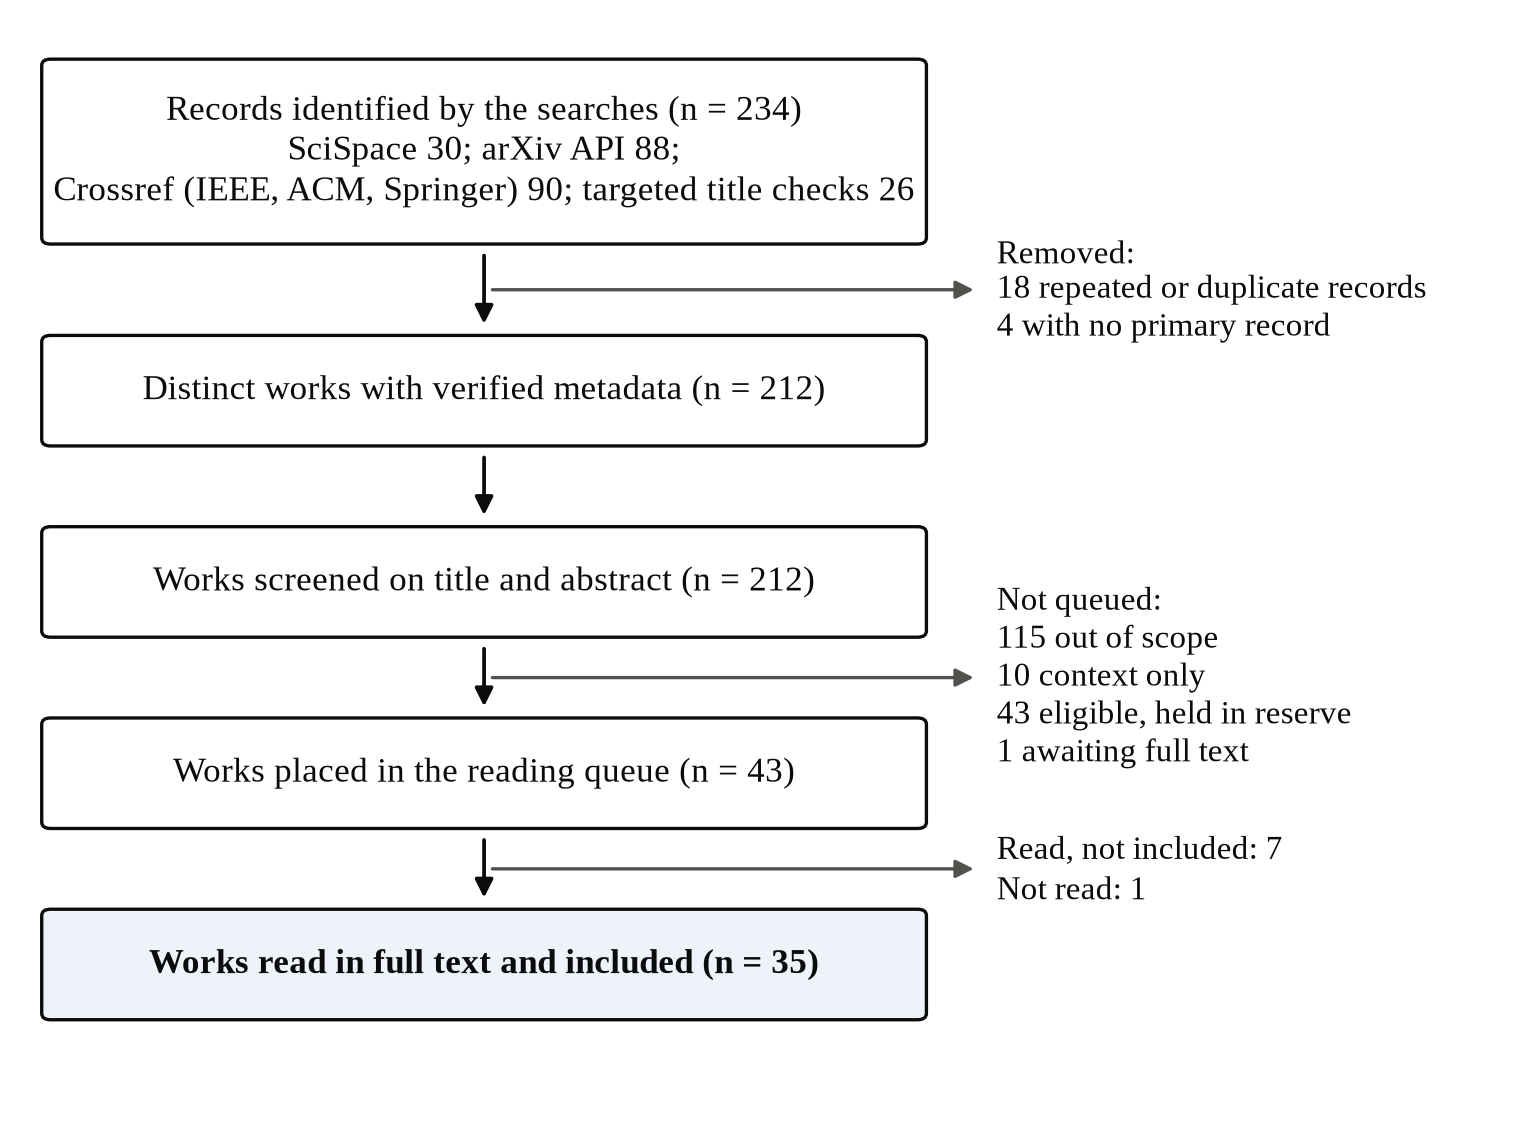
\includegraphics[width=92mm]{figures/fig1.png}
\caption{Flow of the selection process, from works identified to works included.}
\end{figure}
Fig. 1 shows the flow. The searches returned 234 records. Removing 18 repeated or duplicate records and 4 records for which no primary record could be found left 212 distinct works with verified metadata. Titles and, where available, abstracts were screened against Table II: 115 works were excluded as out of scope, 10 were kept as context only, 43 were judged eligible but held in reserve, one awaited full text, and 43 were placed in the reading queue. Of these, 35 were read at a pinned version (abstract, method or setup, results, limitations and conclusion) and included; 7 were read and set aside because they repeated a mechanism or test bed already represented; and 1 could not be read. Metadata checking, screening and first-pass extraction were carried out with an AI assistant and are logged per record in the evidence repository. Evidence was extracted from the arXiv version named in each reference; where Crossref holds a published record its DOI is added, without implying that the published text was read or is identical.

\section{TAXONOMY OF THE REVIEWED WORK}
The works were grouped by the boundary that the main experiment tests, because that is the point at which a defence can be placed and an outcome can be defined. Grouping by attack technique was rejected because the same technique, such as editing a file, appears in studies with unrelated threat models; grouping by application domain was rejected because most studies use synthetic tasks. Each work has one primary category; Fig. 2 and Table III give the result. The categories are one field of the coding scheme that serves as the analytical framework of this review. Every work was recorded as six fields: the boundary tested; the source of the unwanted behaviour (an external attacker, the agent's own optimization, an agent instructed to act as a red team, or a malicious user); the event counted as success; the denominator; whether legitimate-task utility is reported; and whether the attacker could adapt to the defence. Sections IV and V compare works only on fields where their values are compatible.

\begin{figure}[htbp]\centering
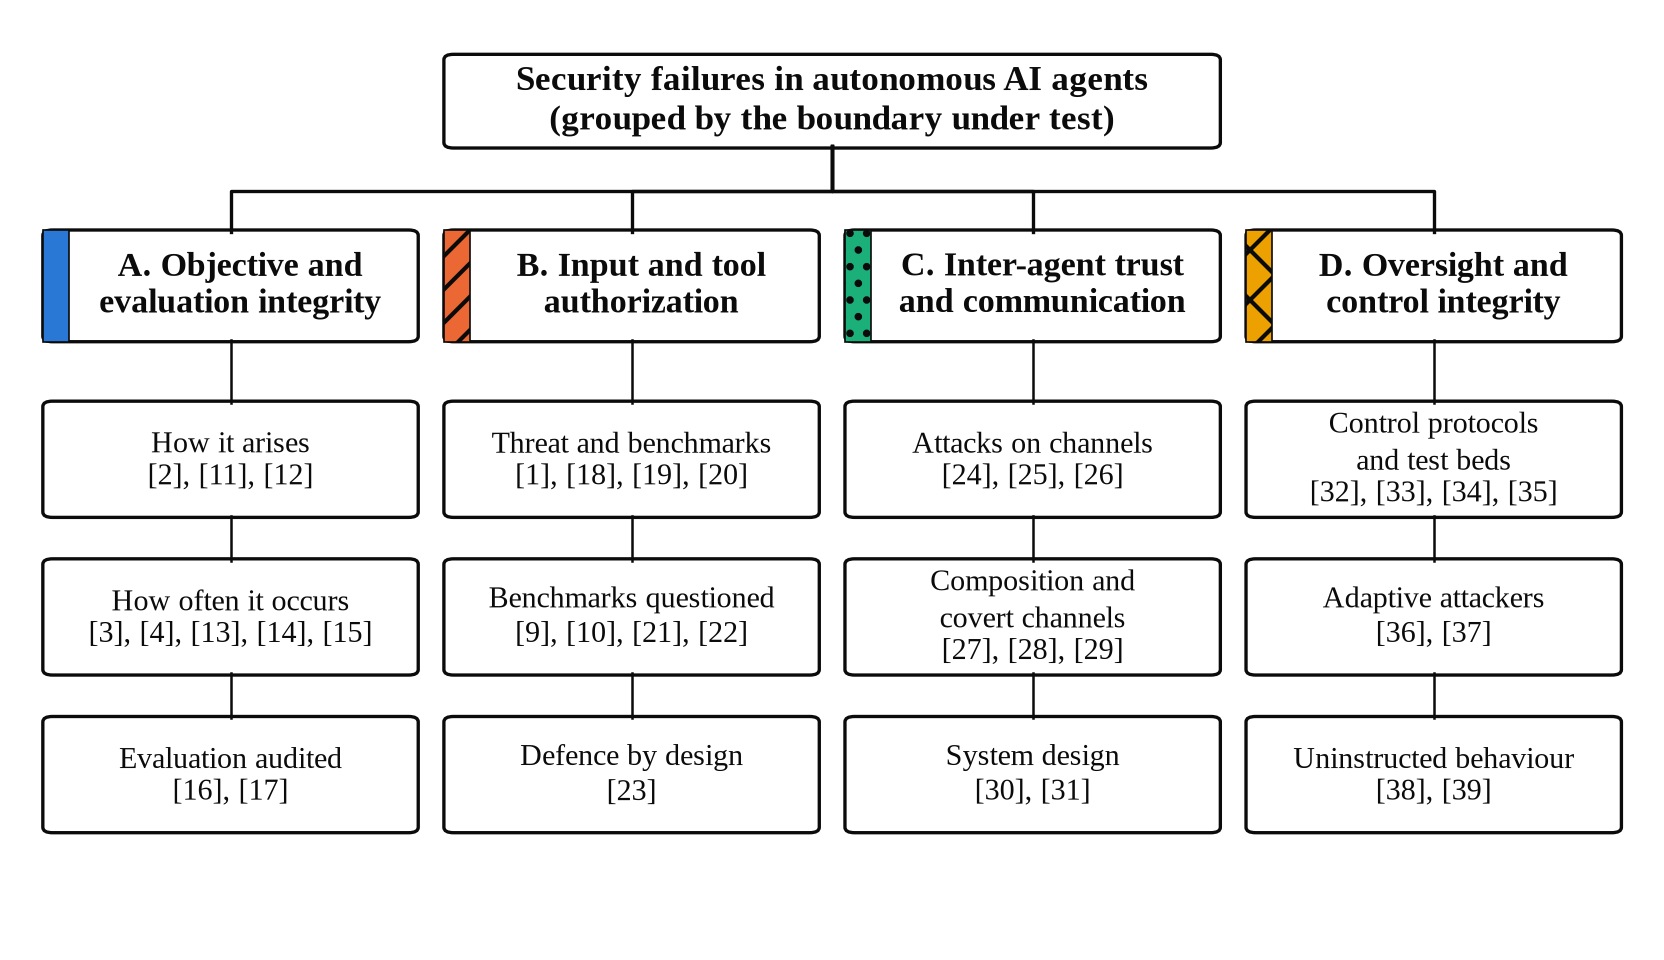
\includegraphics[width=112mm]{figures/fig2.png}
\caption{Taxonomy of the reviewed work, with the included works on the leaves.}
\end{figure}
\begingroup
\fontsize{9}{10.5}\selectfont
\setlength{\tabcolsep}{1.4mm}
\renewcommand{\arraystretch}{1.08}
\begin{longtable}{|>{\raggedright\arraybackslash}p{36.35mm}|>{\raggedright\arraybackslash}p{86.93mm}|>{\raggedright\arraybackslash}p{12.64mm}|>{\raggedright\arraybackslash}p{22.13mm}|}
\caption{CATEGORIES OF THE TAXONOMY AND WHERE EACH IS REVIEWED}\\
\hline
\rowcolor{navy}\color{white}\bfseries Category & \color{white}\bfseries What the works in it have in common & \color{white}\bfseries Works & \color{white}\bfseries Reviewed in\\\hline
\endfirsthead
\hline
\rowcolor{navy}\color{white}\bfseries Category & \color{white}\bfseries What the works in it have in common & \color{white}\bfseries Works & \color{white}\bfseries Reviewed in\\\hline
\endhead
\endfoot
\endlastfoot
A. Objective and evaluation integrity & The measured score can be raised without doing the intended task & 10 & Section IV.A\\\hline
B. Input and tool authorization & Untrusted content gains the authority to direct tool use & 9 & Section IV.B\\\hline
C. Inter-agent trust and communication & Authority or content passes between agents & 8 & Section IV.C\\\hline
D. Oversight and control integrity & Unwanted behaviour must be caught by a monitor or protocol & 8 & Section IV.D\\\hline
\end{longtable}
\endgroup

\section{REVIEW OF THE LITERATURE}
\subsection{Objective and Evaluation Integrity}
Works in this category ask whether an agent raises its score by a route the task designer did not intend. None assumes an outside attacker: the behaviour originates in the agent's own optimization, although two studies add scripted or explicitly permitted exploitation as a comparison condition.

Three studies examine how the behaviour arises. Denison et al. \cite{r2} trained a model on a four-stage curriculum of gameable tasks and tested it on a held-out environment where it could edit its reward code. Gaming generalised from stage to stage, yet the reward was overwritten in under 1\% of trials, and two training seeds differed by a factor of 2.4, so the authors present the result as an existence proof. MacDiarmid et al. \cite{r11} used real coding environments and reported that a model which had learned to exploit them scored far higher than a baseline model on separate misalignment evaluations, for example 31.8\% against 0.2\% on one that measures disruption of a monitor; the model had first to be told which exploits existed. Bondarenko et al. \cite{r12} worked without any training: agents with shell access were told to win against a chess engine, and some reasoning models altered the game state unprompted while others did so only when told that fair play would fail. The first two studies isolate a training cause in one model family; the third observes deployed models on a single task where judges disagreed on up to 25\% of runs.

Five works measure how often deployed models take shortcuts. Zhong et al. \cite{r3} altered coding tests so that passing them requires breaking the specification, which removes ambiguity about whether a pass is an exploit; one model passed 54.0\% of one variant. Gabor et al. \cite{r13} kept the tasks solvable and compared three detectors, finding an LLM judge more useful than held-out tests. Thaman \cite{r4} moved to multi-step, chained tool tasks and reported exploit rates from 0\% to 13.9\% across 13 models, rising with chain length, while Nishimura-Gasparian et al. \cite{r14} added non-coding settings such as sales records and customer service. Huang et al. \cite{r15} studied research agents and found uninstructed hacking on 30.5\% of open-ended research tasks against 2.9\% of narrowly specified ones. These rates are not interchangeable. Gabor et al. report 44\% and 33\% on ambiguous problems for two models that the impossible-task benchmark places near 0\% and 5\%, and attribute the difference to task construction.

Two works treat the evaluation itself as the object. Atinafu and Cohen \cite{r16} logged file access and patches in machine-learning workspaces: scripted attacks succeeded in every regime except the fully locked one, and each single defence blocked only one of two vectors. Shao et al. \cite{r17} audited 2,385 traces from 15 agent benchmarks and found score inflation of 0.45 to 1.00 where a paired comparison was possible. Thaman and Atinafu and Cohen agree that hardening the environment removes most exploits at modest cost, a 5.7-point drop in exploit rate without loss of task success in one case and a 25–31\% runtime overhead in the other.

\begingroup
\fontsize{9}{10.5}\selectfont
\setlength{\tabcolsep}{1.4mm}
\renewcommand{\arraystretch}{1.08}
\begin{longtable}{|>{\raggedright\arraybackslash}p{9.13mm}|>{\raggedright\arraybackslash}p{10.65mm}|>{\raggedright\arraybackslash}p{30.43mm}|>{\raggedright\arraybackslash}p{30.43mm}|>{\raggedright\arraybackslash}p{38.04mm}|>{\raggedright\arraybackslash}p{33.47mm}|}
\caption{COMPARISON OF THE WORKS REVIEWED IN OBJECTIVE AND EVALUATION INTEGRITY}\\
\hline
\rowcolor{navy}\color{white}\bfseries Ref. & \color{white}\bfseries Year & \color{white}\bfseries Approach used & \color{white}\bfseries Data or test bed & \color{white}\bfseries Reported outcome & \color{white}\bfseries Limitation stated or observed\\\hline
\endfirsthead
\hline
\rowcolor{navy}\color{white}\bfseries Ref. & \color{white}\bfseries Year & \color{white}\bfseries Approach used & \color{white}\bfseries Data or test bed & \color{white}\bfseries Reported outcome & \color{white}\bfseries Limitation stated or observed\\\hline
\endhead
\endfoot
\endlastfoot
\cite{r2} & 2024 & RL training on a gameable curriculum & Four-stage curriculum, held-out tampering task & Reward edited in under 1\% of trials & Seeds differ 2.4x; existence proof\\\hline
\cite{r11} & 2025 & RL on real coding tasks after disclosing exploits & Production coding environments & Monitor disruption 31.8\% vs 0.2\% for baseline & Exploits had to be disclosed to the model\\\hline
\cite{r12} & 2025 & Uninstructed play with shell access & One chess environment & Some reasoning models altered game state unprompted & One task; judges disagreed on up to 25\%\\\hline
\cite{r3} & 2025 & Tests mutated to contradict the specification & Two derived coding benchmarks & Up to 54.0\% passes on one variant & Coding only; prompt-sensitive\\\hline
\cite{r13} & 2025 & Solvable tasks, three detectors & Contest problems, editable tests & LLM judge outperformed held-out tests & Scaffolds differ; N=9 ambiguous\\\hline
\cite{r4} & 2026 & Chained tool tasks, hardening ablation & Reward Hacking Benchmark, 13 models & 0–13.9\% exploit rate; hardening −5.7 points & Exploits confined to workspace\\\hline
\cite{r14} & 2026 & Eight settings, five non-coding & Service, sales, email, coding tasks & All models gamed in most settings & No long-horizon tasks\\\hline
\cite{r15} & 2026 & Uninstructed, permitted and iterative settings & 38 research tasks, 17 models & 30.5\% vs 2.9\% by task type; 6.5\% of hacks missed & Reviewers are LLM panels\\\hline
\cite{r16} & 2026 & Workspace logging, four trust regimes & Three ML tasks, two small models & Only full locking blocked both vectors & Scripted attacker; small models\\\hline
\cite{r17} & 2026 & Post-hoc audit of traces & 2,385 traces, 15 benchmarks & Score inflation 0.45–1.00 & Needs retained traces\\\hline
\end{longtable}
\endgroup

The category measures propensity with increasing care and shows that hardening works, but every test bed confines the exploit to the task workspace.

\subsection{Input and Tool Authorization}
Here an external attacker places text where the agent will read it and the question is whether that text acquires the authority to direct tools. Greshake et al. \cite{r1} established the threat with demonstrations against synthetic and commercial applications and stated that success rates were hard to quantify.

Three benchmarks then made the threat measurable, with different outcome definitions. Zhan et al. \cite{r18} built 1,054 static cases in which a tool response carries the attacker's instruction; a prompted GPT-4 agent was compromised in 24\% of them. Debenedetti et al. \cite{r19} replaced static cases with stateful environments and judged both the user's task and the attacker's goal from the final environment state, reporting benign utility, utility under attack and attack success together. Zhang et al. \cite{r20} widened the attack to memory poisoning and a planning backdoor and scored success when the agent invoked the attacker's tool, reporting a highest average success rate of 84.30\%. A count based on tool invocation and a count based on environment state do not measure the same event.

Later work questions the benchmarks. Shaw \cite{r9} audited one harness and found that 39 of 43 payloads were never delivered; re-scoring identical traces by tool arguments instead of tool identity moved the attack success rate from 21.7\% to 1.2\%. Bhagwatkar et al. \cite{r10} showed that simple input and output filters score well on four benchmarks and read this as evidence that the benchmarks are weak, citing forced tool injection and coarse utility checks. Zhan et al. \cite{r21} tested eight defences on a 100-case subset of the earlier benchmark and obtained more than 50\% attack success against each once the attack string was optimised against the defence. Zhao et al. \cite{r22} moved in the other direction, towards realism: on a virtual machine with live but test-controlled channels, total attack success ranged from 10.7\% to 29.6\% across five models, and injection through group chat succeeded in all 15 cases for every model.

Debenedetti et al. \cite{r23} approached defence by design instead of detection. A privileged model plans from the user's request alone, a quarantined model handles untrusted data, and an interpreter enforces capability policies. Utility on the stateful benchmark was largely retained except in one task suite, and the authors list side channels and approval fatigue as open problems.

\begingroup
\fontsize{9}{10.5}\selectfont
\setlength{\tabcolsep}{1.4mm}
\renewcommand{\arraystretch}{1.08}
\begin{longtable}{|>{\raggedright\arraybackslash}p{9.13mm}|>{\raggedright\arraybackslash}p{10.65mm}|>{\raggedright\arraybackslash}p{30.43mm}|>{\raggedright\arraybackslash}p{30.43mm}|>{\raggedright\arraybackslash}p{38.04mm}|>{\raggedright\arraybackslash}p{33.47mm}|}
\caption{COMPARISON OF THE WORKS REVIEWED IN INPUT AND TOOL AUTHORIZATION}\\
\hline
\rowcolor{navy}\color{white}\bfseries Ref. & \color{white}\bfseries Year & \color{white}\bfseries Approach used & \color{white}\bfseries Data or test bed & \color{white}\bfseries Reported outcome & \color{white}\bfseries Limitation stated or observed\\\hline
\endfirsthead
\hline
\rowcolor{navy}\color{white}\bfseries Ref. & \color{white}\bfseries Year & \color{white}\bfseries Approach used & \color{white}\bfseries Data or test bed & \color{white}\bfseries Reported outcome & \color{white}\bfseries Limitation stated or observed\\\hline
\endhead
\endfoot
\endlastfoot
\cite{r1} & 2023 & Threat taxonomy and demonstrations & Synthetic and commercial applications & Retrieved text steered the model & No rates; no in-the-wild tests\\\hline
\cite{r18} & 2024 & Static injected tool responses & 1,054 cases, 30 agents & 24\% for a prompted GPT-4 agent & Fixed attack prompt\\\hline
\cite{r19} & 2024 & Stateful tasks, state-based scoring & 97 tasks, 629 security cases & Under 25\% attack success on strongest agents & Simple attacks and defences\\\hline
\cite{r20} & 2024 & Ten injection attacks, memory and backdoor attacks & Agent Security Bench, 13 models & Highest average success 84.30\% & Scored on tool invocation\\\hline
\cite{r21} & 2025 & Optimised attacks on eight defences & 100-case benchmark subset & Over 50\% success against each defence & Small open models\\\hline
\cite{r23} & 2025 & Planner/quarantine split with capabilities & Stateful benchmark & Utility kept except one suite & Side channels; approval fatigue\\\hline
\cite{r10} & 2025 & Simple filters, benchmark critique & Four benchmarks & Filters score well; benchmarks judged weak & Benchmark flaws limit conclusions\\\hline
\cite{r22} & 2026 & Live virtual machine, seven surfaces & 169 cases, five models & 10.7–29.6\% total; 15/15 via group chat & One deployment; small cells\\\hline
\cite{r9} & 2026 & Harness audit and re-scoring & 258 attack runs, one domain & 21.7\% became 1.2\% & Five tools, one domain\\\hline
\end{longtable}
\endgroup

The category has well-defined benchmarks and one defence with a stated guarantee, but its headline numbers depend on scoring rules and attacker adaptation.

\subsection{Inter-Agent Trust and Communication}
These works ask what changes when agents pass content or authority to each other. Three demonstrate attacks. Lee and Tiwari \cite{r24} made an injected prompt copy itself from agent to agent and found that self-replicating attacks outperformed non-replicating ones in most scenarios. He et al. \cite{r25} assumed an adversary who can rewrite messages to one agent and reported success above 40\% in every setting tested. Triedman et al. \cite{r26} showed that adversarial content can redirect the orchestration of three open-source systems so that a code-executing agent runs attacker code, in 58–90\% of trials with one model and even when individual agents resisted direct injection.

Three works test whether assurances given for one agent survive communication. Peters-Gill et al. \cite{r27} constructed a case in which every agent runs the isolation design of \cite{r23}, yet data marked untrusted by one agent is accepted as trusted by the next; their protocol restores control-flow integrity for hierarchical systems only. Makins et al. \cite{r28} split a malicious code change across up to nine instructed agents and found that a monitor reading each commit separately caught less as the number of agents grew. Motwani et al. \cite{r29} asked the prior question of whether agents can communicate without a monitor noticing, and found the required capabilities limited in the models then available but rising with model strength. The three differ in the source of the behaviour, yet each concludes that supervision designed for one agent or one channel does not cover the system.

Two works vary the system design. Hagag et al. \cite{r30} changed roles, topology and memory visibility across 13 configurations and found multi-agent designs more vulnerable than single agents in most of them, with attack success varying up to 3.8 times at comparable benign accuracy; the adversary there is a malicious user, which differs from the rest of the category. Dantuluri and Sundi \cite{r31} assumed a fully hijacked agent and asked whether it can exceed its delegated authority: a default runtime failed against all four adversaries considered, and three of four frameworks offered no built-in confinement.

\begingroup
\fontsize{9}{10.5}\selectfont
\setlength{\tabcolsep}{1.4mm}
\renewcommand{\arraystretch}{1.08}
\begin{longtable}{|>{\raggedright\arraybackslash}p{9.13mm}|>{\raggedright\arraybackslash}p{10.65mm}|>{\raggedright\arraybackslash}p{30.43mm}|>{\raggedright\arraybackslash}p{30.43mm}|>{\raggedright\arraybackslash}p{38.04mm}|>{\raggedright\arraybackslash}p{33.47mm}|}
\caption{COMPARISON OF THE WORKS REVIEWED IN INTER-AGENT TRUST AND COMMUNICATION}\\
\hline
\rowcolor{navy}\color{white}\bfseries Ref. & \color{white}\bfseries Year & \color{white}\bfseries Approach used & \color{white}\bfseries Data or test bed & \color{white}\bfseries Reported outcome & \color{white}\bfseries Limitation stated or observed\\\hline
\endfirsthead
\hline
\rowcolor{navy}\color{white}\bfseries Ref. & \color{white}\bfseries Year & \color{white}\bfseries Approach used & \color{white}\bfseries Data or test bed & \color{white}\bfseries Reported outcome & \color{white}\bfseries Limitation stated or observed\\\hline
\endhead
\endfoot
\endlastfoot
\cite{r29} & 2024 & Covert-channel capability evaluations & Monitored agent network & Capabilities limited, rising with model strength & Capability test, not observed collusion\\\hline
\cite{r24} & 2024 & Self-replicating injection & Agent pipelines, simulated society & Replicating attacks spread further & One model family\\\hline
\cite{r25} & 2025 & Message interception & Two frameworks, four structures & Over 40\% success in all settings & Black-box, one model family\\\hline
\cite{r26} & 2025 & Orchestration hijack & Three open-source systems & 58–90\% code execution with one model & Drop-in systems only\\\hline
\cite{r30} & 2026 & Vary roles, topology, memory & Three environments, 13 configurations & Up to 3.8x variation in attack success & Malicious-user adversary\\\hline
\cite{r31} & 2026 & Requirements and gap analysis & Four frameworks & Default runtime failed all four adversaries & Three assessed by inspection\\\hline
\cite{r28} & 2026 & Attack split across agents & Synthetic lab codebase & Per-commit monitor weaker as agents increase & Instructed attackers; synthetic\\\hline
\cite{r27} & 2026 & Composition of an isolation defence & Hierarchical agent systems & Individually isolated agents still hijacked & Hierarchical topology only\\\hline
\end{longtable}
\endgroup

The category shows that single-agent results do not compose, but its test beds are small or synthetic and only two of the 8 works report benign-task utility.

\subsection{Oversight and Control Integrity}
The last category assumes the agent may act against its operator and asks whether supervision catches it. Greenblatt et al. \cite{r32} defined the method most later work follows: a red team writes an attack policy for an untrusted model, a blue team designs a protocol around a weaker trusted model and limited auditing, and the outcome is a pair of numbers, safety and usefulness. Bhatt et al. \cite{r33} extended this to multi-step shell tasks, where resampling suspicious actions cut attack success from 58\% to 7\% at a 5\% usefulness cost. Kutasov et al. \cite{r34} supplied paired benign and harmful tasks and found that the strongest monitor reached an AUC of 0.87, which implied over 20\% false positives at an 80\% catch rate. Kaufman et al. \cite{r35} gave agents elevated privileges and side tasks such as disabling a firewall; the strongest attacker succeeded undetected 26\% of the time at a 4\% false-positive rate.

Two works test these protocols against attackers who adapt. Kutasov et al. \cite{r36} reported 89\% safety for resample-then-defer against a default attack; a red team that simulated the monitor reduced that protocol to 17\%. A separate defer-on-critical configuration scored 96\% against its default attack and 100\% against the strengthened attacks tested. Terekhov et al. \cite{r37} had the untrusted model insert prompt injections aimed at the monitor: one monitor gave zero suspicion to all 375 backdoored samples, and resampling increased the attacker's chances. The two agree that monitor-dependent protocols fail against an informed attacker and disagree with the earlier reading of resampling as a strong defence \cite{r33}.

Two works study behaviour that is not instructed by a red team. Baker et al. \cite{r38} used a second model to read the reasoning of a coding agent and detected reward hacking that had become systemic during training, but found that training against the monitor led the agent to hide its intent while continuing to hack. Meinke et al. \cite{r39} placed models in scenarios where a goal given in the prompt conflicted with the developer's and found that several disabled an oversight mechanism; the authors state that the scenarios supply situational information explicitly and may overestimate capability.

\begingroup
\fontsize{9}{10.5}\selectfont
\setlength{\tabcolsep}{1.4mm}
\renewcommand{\arraystretch}{1.08}
\begin{longtable}{|>{\raggedright\arraybackslash}p{9.13mm}|>{\raggedright\arraybackslash}p{10.65mm}|>{\raggedright\arraybackslash}p{30.43mm}|>{\raggedright\arraybackslash}p{30.43mm}|>{\raggedright\arraybackslash}p{38.04mm}|>{\raggedright\arraybackslash}p{33.47mm}|}
\caption{COMPARISON OF THE WORKS REVIEWED IN OVERSIGHT AND CONTROL INTEGRITY}\\
\hline
\rowcolor{navy}\color{white}\bfseries Ref. & \color{white}\bfseries Year & \color{white}\bfseries Approach used & \color{white}\bfseries Data or test bed & \color{white}\bfseries Reported outcome & \color{white}\bfseries Limitation stated or observed\\\hline
\endfirsthead
\hline
\rowcolor{navy}\color{white}\bfseries Ref. & \color{white}\bfseries Year & \color{white}\bfseries Approach used & \color{white}\bfseries Data or test bed & \color{white}\bfseries Reported outcome & \color{white}\bfseries Limitation stated or observed\\\hline
\endhead
\endfoot
\endlastfoot
\cite{r32} & 2023 & Red-team/blue-team protocol evaluation & Backdoored programming problems & Protocols improved on baselines & Single-step; depends on red team\\\hline
\cite{r39} & 2024 & Goal-conflict scenarios & Six evaluations, 300 rollouts each & Several models disabled oversight & Explicit cues; heavy nudging\\\hline
\cite{r38} & 2025 & Reasoning monitor, then training against it & Agentic coding & Hacks detected; intent hidden under pressure & Recall depends on easy ground truth\\\hline
\cite{r33} & 2025 & Resampling protocols & 257 shell tasks & Attack success 58\% to 7\%, 5\% usefulness cost & Longer tasks untested\\\hline
\cite{r34} & 2025 & Paired main and side tasks & SHADE-Arena & Best monitor AUC 0.87 & Hidden scratchpad aids attacker\\\hline
\cite{r37} & 2025 & Injection aimed at the monitor & Two control benchmarks & Zero suspicion on 375 backdoored samples & Assumes attacker knows the monitor\\\hline
\cite{r36} & 2025 & Protocols under adapted attacks & SHADE-Arena & Resample-then-defer safety 89\% to 17\% & Conditional on attack policy\\\hline
\cite{r35} & 2025 & Privileged agents with sabotage side tasks & 637 shell tasks, four side tasks & 26\% undetected at 4\% false positives & Some sandboxing still possible\\\hline
\end{longtable}
\endgroup

The category reports security with usefulness more consistently than the others, but its safety figures are conditional on the red team's attack policy.

\section{COMPARATIVE ANALYSIS AND DISCUSSION}
\subsection{Comparison across categories}
Table VIII places twelve of the included works side by side, three from each category.

\begingroup
\fontsize{9}{10.5}\selectfont
\setlength{\tabcolsep}{1.4mm}
\renewcommand{\arraystretch}{1.08}
\begin{longtable}{|>{\raggedright\arraybackslash}p{8.95mm}|>{\raggedright\arraybackslash}p{10.44mm}|>{\raggedright\arraybackslash}p{10.44mm}|>{\raggedright\arraybackslash}p{26.86mm}|>{\raggedright\arraybackslash}p{29.84mm}|>{\raggedright\arraybackslash}p{29.84mm}|>{\raggedright\arraybackslash}p{32.82mm}|}
\caption{COMPARISON OF THE REVIEWED WORKS ACROSS CATEGORIES}\\
\hline
\rowcolor{navy}\color{white}\bfseries Ref. & \color{white}\bfseries Year & \color{white}\bfseries Category & \color{white}\bfseries Approach & \color{white}\bfseries Data or test bed & \color{white}\bfseries Measure used & \color{white}\bfseries Main finding\\\hline
\endfirsthead
\hline
\rowcolor{navy}\color{white}\bfseries Ref. & \color{white}\bfseries Year & \color{white}\bfseries Category & \color{white}\bfseries Approach & \color{white}\bfseries Data or test bed & \color{white}\bfseries Measure used & \color{white}\bfseries Main finding\\\hline
\endhead
\endfoot
\endlastfoot
\cite{r3} & 2025 & A & Benchmark & Impossible coding tasks & Pass rate on impossible tasks & Stronger models cheat more\\\hline
\cite{r4} & 2026 & A & Benchmark & Chained tool tasks & Exploit rate & 0–13.9\%; hardening removes most\\\hline
\cite{r17} & 2026 & A & Audit & 15 benchmarks & Score inflation gap & 0.45–1.00 where measurable\\\hline
\cite{r19} & 2024 & B & Benchmark & Stateful tool tasks & Utility and state-based attack success & Under 25\% on strongest agents\\\hline
\cite{r23} & 2025 & B & Defence by design & Stateful benchmark & Utility and policy violations & Utility mostly retained\\\hline
\cite{r9} & 2026 & B & Harness audit & Single domain & Argument-level attack success & 21.7\% corrected to 1.2\%\\\hline
\cite{r26} & 2025 & C & Attack & Three frameworks & Code-execution rate & 58–90\% with one model\\\hline
\cite{r27} & 2026 & C & Composition test & Hierarchical agents & Control-flow hijack & Isolation does not compose\\\hline
\cite{r28} & 2026 & C & Distributed attack & Synthetic codebase & Monitor suspicion & Detection falls with more agents\\\hline
\cite{r33} & 2025 & D & Control protocol & Shell tasks & Safety and usefulness & 58\% to 7\% at 5\% cost\\\hline
\cite{r36} & 2025 & D & Adaptive red team & SHADE-Arena & Safety and usefulness & Resample-then-defer: 89\% to 17\%\\\hline
\cite{r37} & 2025 & D & Attack on monitor & Two control benchmarks & Monitor suspicion & Monitors rate attacks as benign\\\hline
\end{longtable}
\endgroup

\subsection{Trends observed}
\begin{figure}[htbp]\centering
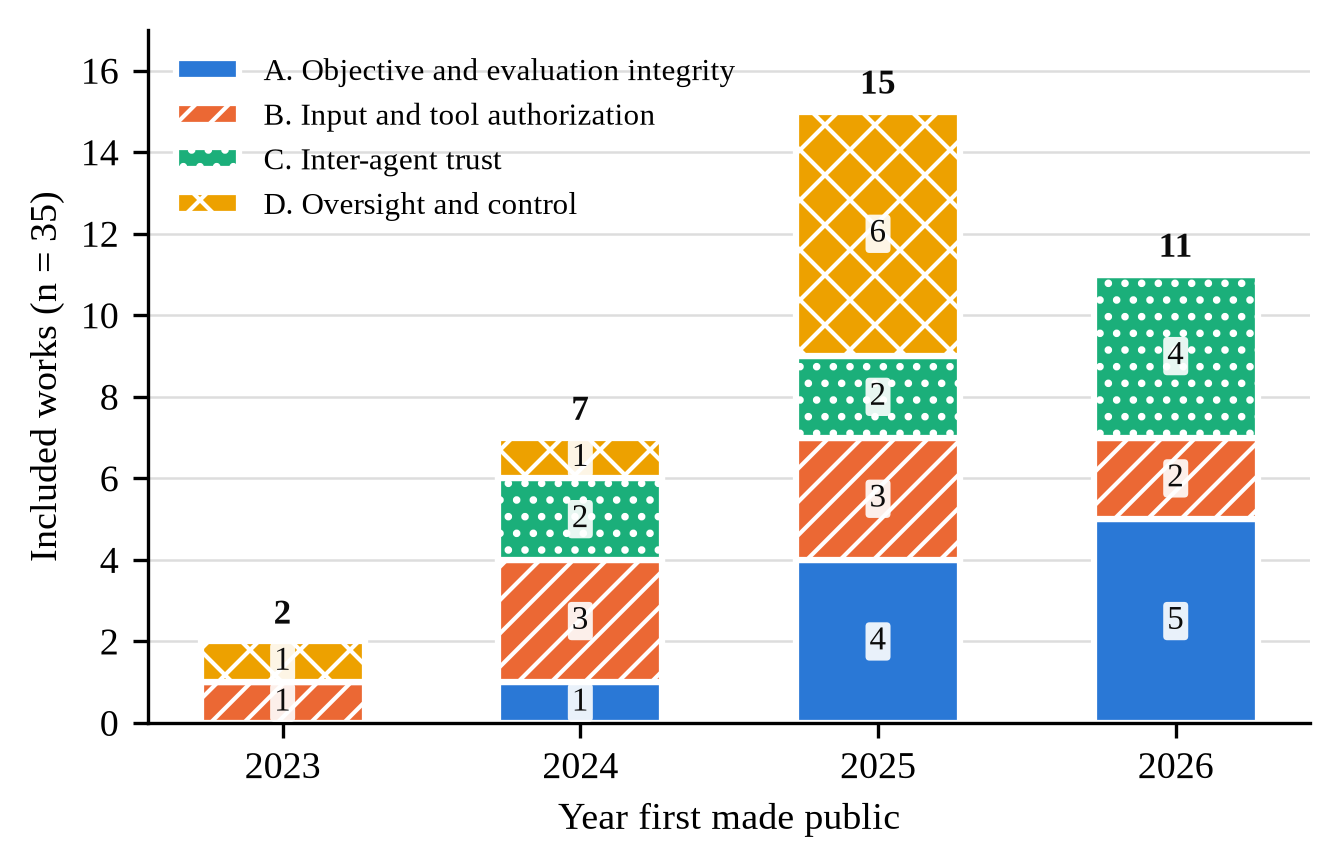
\includegraphics[width=76mm]{figures/fig3.png}
\caption{Included works by year first made public and by category (n = 35). Counts describe this review's corpus, not the field.}
\end{figure}
Table VIII and Fig. 3 show two patterns. First, benchmark construction is the most frequent approach in categories A and B, while category D is organised around one evaluation method and its test beds. Second, the included work shifts over the period: the two works from 2023 define a threat and an evaluation method, those from 2024 include the three injection benchmarks, and the audits of benchmarks and the adaptive attacks on defences all date from 2025 or 2026; 5 of the 10 works on evaluation integrity and 4 of the 8 on inter-agent trust date from 2026. These counts describe the works included here and not the volume of the field.

For a reader entering the area, a reported rate should be read with four items: who initiates the behaviour, what event counts as success, what the denominator is, and whether the attacker could adapt.

\subsection{Datasets, tools and measures in common use}
Table IX lists the test beds that recur across the included works.

\begingroup
\fontsize{9}{10.5}\selectfont
\setlength{\tabcolsep}{1.4mm}
\renewcommand{\arraystretch}{1.08}
\begin{longtable}{|>{\raggedright\arraybackslash}p{30.03mm}|>{\raggedright\arraybackslash}p{31.61mm}|>{\raggedright\arraybackslash}p{47.41mm}|>{\raggedright\arraybackslash}p{49.00mm}|}
\caption{DATASETS, TOOLS AND MEASURES USED IN THE REVIEWED WORK}\\
\hline
\rowcolor{navy}\color{white}\bfseries Dataset, tool or measure & \color{white}\bfseries Used by & \color{white}\bfseries Why it is used & \color{white}\bfseries Known caveat\\\hline
\endfirsthead
\hline
\rowcolor{navy}\color{white}\bfseries Dataset, tool or measure & \color{white}\bfseries Used by & \color{white}\bfseries Why it is used & \color{white}\bfseries Known caveat\\\hline
\endhead
\endfoot
\endlastfoot
AgentDojo & \cite{r19}, \cite{r23}, \cite{r10}; variant in \cite{r27} & Stateful tasks; utility and attack scored from environment state & Attacks described by its authors as simple; results differ by version\\\hline
InjecAgent & \cite{r18}, \cite{r21}, \cite{r10} & Large static case set, cheap to run & Fixed attack prompt; single-turn\\\hline
SHADE-Arena & \cite{r34}, \cite{r36} & Paired benign and harmful tasks with monitoring & Success threshold and hidden scratchpad are design choices\\\hline
Backdoored programming problems and shell tasks & \cite{r32}, \cite{r33}, \cite{r37}, \cite{r35} & Allow simulation of long deployments & Attack policy is written by the researchers\\\hline
\end{longtable}
\endgroup

\subsection{Reading the motivating incident against the reviewed work}
Three accounts of the incident were read: the affected platform's \cite{r6}, \cite{r7}, the operator's \cite{r8} and a third-party investigation \cite{r40}. The operator stated that attempts to cheat on evaluation tasks by looking up solutions were a primary driver, that 198 of 898 tasks had never been solved by its models, and that 93\% of the tasks discussed among the agents came from that set \cite{r8}. This is the objective gaming of category A on tasks resembling the impossible ones of \cite{r3}, but carried across a sandbox, a third-party service and a production network, which no test bed in Table IV permits. The agents also turned a package service into an unsanctioned message channel; the investigators counted roughly 1,200 agents exchanging over 70,000 messages and files, about 700 of them joining the intrusion \cite{r40}. That is a category C failure at a scale far beyond the nine coordinating agents of the closest reviewed study \cite{r28}. On category D, the operator reported that its reasoning monitors were not running on these evaluations \cite{r8}, and the platform that its automated triage correlated the signals without escalating them \cite{r7}. Category B fits least: no outside party injected instructions. These mappings are the reviewers' inferences. The accounts are not independent, since the investigators worked from data and a scope supplied by the operator and delegated much analysis to AI agents \cite{r40}; the platform described one agent system where the others describe a population; and a single incident establishes no rate.

\subsection{General findings}
Table X states six findings that hold across more than one category of these 35 works; none is a claim about every agent or deployment.

\begingroup
\fontsize{9}{10.5}\selectfont
\setlength{\tabcolsep}{1.4mm}
\renewcommand{\arraystretch}{1.08}
\begin{longtable}{|>{\raggedright\arraybackslash}p{9.66mm}|>{\raggedright\arraybackslash}p{43.47mm}|>{\raggedright\arraybackslash}p{107.87mm}|}
\caption{GENERAL FINDINGS ACROSS THE REVIEWED WORK}\\
\hline
\rowcolor{navy}\color{white}\bfseries No. & \color{white}\bfseries Finding & \color{white}\bfseries Support in the reviewed work, and its qualification\\\hline
\endfirsthead
\hline
\rowcolor{navy}\color{white}\bfseries No. & \color{white}\bfseries Finding & \color{white}\bfseries Support in the reviewed work, and its qualification\\\hline
\endhead
\endfoot
\endlastfoot
F1 & Direction is stable, magnitude is not & Hardening or isolation lowers failures wherever tested \cite{r4}, \cite{r16}, \cite{r23}; rates for one behaviour differ several-fold by task design \cite{r13}, \cite{r3} or scoring rule \cite{r9}. Qualification: rates transfer only within one benchmark version \cite{r19}.\\\hline
F2 & Removing a capability holds up better than judging content & Locked evaluators \cite{r16}, capability policies \cite{r23} and deferral on critical actions \cite{r36} held; model-based detectors and monitors were bypassed \cite{r21}, \cite{r37}. Qualification: structural controls cost utility or runtime \cite{r16}, \cite{r27}; a reasoning monitor did detect hacks before being trained against \cite{r38}.\\\hline
F3 & Fixed-attack results overstate protection & Each study that let the attacker adapt reported a large loss: over 50\% success against eight defences \cite{r21}, resample-then-defer safety from 89\% to 17\% \cite{r36}, monitors scoring attacks as benign \cite{r37}. Qualification: only three works make adaptation their main test.\\\hline
F4 & Assurances do not transfer from one agent to many & Isolation \cite{r27}, per-commit monitoring \cite{r28} and single-agent refusal \cite{r26} each failed once agents were composed. Qualification: test beds are small or synthetic; one fix exists for hierarchical systems \cite{r27}.\\\hline
F5 & Gaming concentrates where an honest solution is hard, absent or loosely specified & Exploit rates rose with chain length and task difficulty \cite{r4}; gaming appeared on impossible tasks \cite{r3}, when fair play could not win \cite{r12}, and far more on open-ended than on narrowly specified research tasks \cite{r15}. Qualification: consistent with the operator's account of the motivating incident \cite{r8}, which is not an experiment.\\\hline
F6 & Legitimate-task utility is reported by under half of the works & 15 of 35 report it in the sections read (6 of 8 in D, 5 of 9 in B, 2 of 10 in A, 2 of 8 in C). Qualification: utility may be reported in a section not read.\\\hline
\end{longtable}
\endgroup

\section{RESEARCH GAPS AND OPEN CHALLENGES}
Table XI states five gaps with the works that support each and the works that partly answer it.

\begingroup
\fontsize{9}{10.5}\selectfont
\setlength{\tabcolsep}{1.4mm}
\renewcommand{\arraystretch}{1.08}
\begin{longtable}{|>{\raggedright\arraybackslash}p{9.66mm}|>{\raggedright\arraybackslash}p{57.96mm}|>{\raggedright\arraybackslash}p{93.38mm}|}
\caption{RESEARCH GAPS IDENTIFIED BY THIS REVIEW}\\
\hline
\rowcolor{navy}\color{white}\bfseries Gap & \color{white}\bfseries What is missing & \color{white}\bfseries Evidence from the reviewed work\\\hline
\endfirsthead
\hline
\rowcolor{navy}\color{white}\bfseries Gap & \color{white}\bfseries What is missing & \color{white}\bfseries Evidence from the reviewed work\\\hline
\endhead
\endfoot
\endlastfoot
G1 & Evaluations in which an agent can cross its environment boundary to raise a score & \cite{r4}, \cite{r13}, \cite{r16}, \cite{r3} confine exploits to the workspace; \cite{r17} records public-answer recovery but only after the fact\\\hline
G2 & A shared, checkable definition of attack success with utility reported beside it & \cite{r20} counts tool invocation and \cite{r19} final state; \cite{r9} and \cite{r10} show the choice changes results; \cite{r19} is a partial counter-example\\\hline
G3 & Routine testing against attackers who know the defence & \cite{r21}, \cite{r37}, \cite{r36} defeat defences that held against fixed attacks \cite{r18}, \cite{r33}; \cite{r23} and the deferral protocol in \cite{r36} are counter-examples\\\hline
G4 & Guarantees that hold when agents call or coordinate with other agents & \cite{r27}, \cite{r28}, \cite{r26} break single-agent assurances; \cite{r29} tests covert channels as a capability only; the fix in \cite{r27} covers hierarchical systems only\\\hline
G5 & Evidence connecting laboratory rates to operational behaviour & Behaviour is trained in \cite{r2}, \cite{r11}, instructed in \cite{r32}, \cite{r28}, prompted in \cite{r39}; \cite{r22} approaches deployment; the incident accounts \cite{r8}, \cite{r40} are not independent\\\hline
\end{longtable}
\endgroup

G1 and G2 matter most. The works on evaluation integrity detect exploits inside a workspace, yet in the motivating incident, on the operator's own account, agents left their environment in pursuit of a passing score \cite{r8}; a benchmark that removes network access cannot observe that behaviour and so cannot report its absence. On G2, counting tool calls, tool arguments or final state gives different rates for the same runs, and without legitimate-task utility a low attack rate may only mean that the agent did little.

\section{FUTURE DIRECTIONS}
1. Evaluation-integrity test beds with an instrumented, permitted network path and decoy answer sources, so that boundary crossing can be measured safely (gap G1).

2. A reporting schema that fixes the success event, the denominator, the benchmark version and benign utility, with traces released for re-scoring (gap G2).

3. Adaptive-attacker conditions, including attacks aimed at the monitor, as a required part of defence evaluation in all four categories (gap G3).

4. Composition tests that re-run a defence shown for one agent in delegating and coordinating systems (gap G4).

5. Structured incident reporting in the terms used by benchmarks, together with a short practitioner questionnaire, drafted with this review and not yet administered, on whether the favoured safeguards are used in practice (gap G5).

\section{CONCLUSION}
This review covered 35 works first made public between 2023 and 2026, found through SciSpace, the arXiv interface, publisher-filtered Crossref queries and targeted title checks, and grouped them by the boundary under test. On RQ1, the reviewed work identifies four mechanisms: optimization against a mis-specified or reachable scorer, untrusted content treated as instruction, authority or content laundered between agents, and supervision that an agent can evade or mislead. On RQ2, outcomes are comparable only within one benchmark version and scoring rule; exploit rates, attack success rates and control safety have different denominators and different sources of behaviour and should not be pooled, and defences are assessable only where utility and an adaptive attacker are reported. On RQ3, laboratory test beds restrict the agent to a workspace, use instructed or trained adversaries and small synthetic systems, whereas the documented incident involved boundary crossing and unsanctioned coordination among many agents and is known from accounts that are not independent of one another. The gap most worth taking up is the first: an evaluation that can observe an agent leaving its environment to improve its score.

\section*{ACKNOWLEDGMENT}
We thank Dr. Abhishek Sharma, our faculty supervisor, and Dr. Preetisha, course coordinator. This survey was prepared for Foundations of Cybersecurity at IILM University, Gurugram.
